% Archetype F3 : schema de mecanisme moleculaire (deletion medieee par IS6110)
% Trois etats successifs du meme locus. Le lecteur doit pouvoir reconstituer
% la CAUSE de l'observation (une RD) et pas seulement constater l'observation.
\documentclass[border=4pt]{standalone}
\usepackage[T1]{fontenc}
\usepackage{lmodern}
\usepackage{xcolor}
\usepackage{tikz}
\usetikzlibrary{positioning,arrows.meta,calc,decorations.pathreplacing,shapes.misc,backgrounds}

\definecolor{isblue}{HTML}{0072B2}
\definecolor{lostred}{HTML}{D55E00}
\definecolor{genegreen}{HTML}{009E73}
\definecolor{neutralgrey}{HTML}{4D4D4D}
\definecolor{backbone}{HTML}{BFBFBF}

\begin{document}
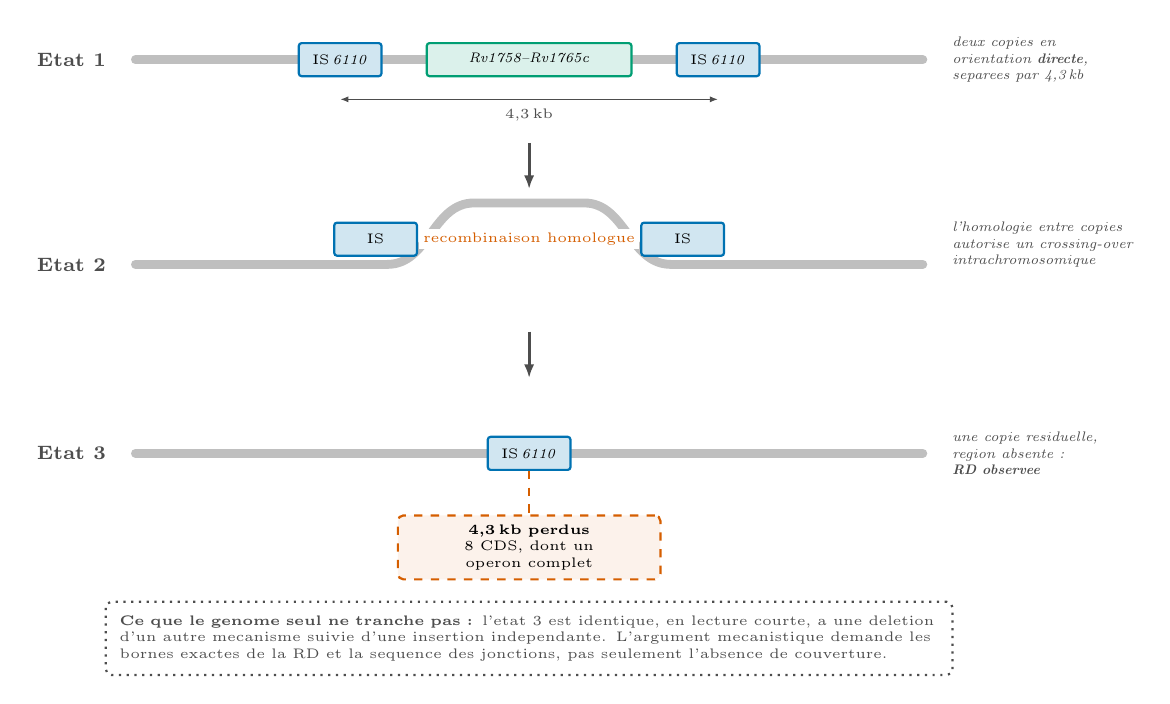
\begin{tikzpicture}[
    every node/.style={font=\scriptsize, align=center},
    chrom/.style={line width=3.2pt, color=backbone, cap=round},
    is/.style={
      draw=isblue, fill=isblue!18, thick,
      minimum height=0.42cm, minimum width=1.05cm, inner sep=1pt,
      font=\tiny, rounded corners=1pt
    },
    gene/.style={
      draw=genegreen, fill=genegreen!14, thick,
      minimum height=0.42cm, inner sep=2pt, font=\tiny, rounded corners=1pt
    },
    stepflow/.style={-{Latex[length=5pt]}, line width=1pt, neutralgrey, shorten >=3pt, shorten <=3pt},
    lab/.style={font=\tiny\itshape, text=neutralgrey, align=left},
    state/.style={font=\scriptsize\bfseries, anchor=east, text=neutralgrey}
  ]

  % ---------- etat 1 : deux copies d'IS en orientation directe -------------
  \draw[chrom] (0,0) -- (10,0);
  \node[is]   (isa) at (2.6,0) {IS\,\emph{6110}};
  \node[is]   (isb) at (7.4,0) {IS\,\emph{6110}};
  \node[gene, minimum width=2.6cm] (rdgene) at (5.0,0) {\emph{Rv1758--Rv1765c}};
  \node[state] at (-0.25,0) {Etat 1};
  \node[lab, anchor=west] at (10.25,0) {deux copies en\\orientation \textbf{directe},\\separees par 4{,}3\,kb};
  \draw[{Latex[length=3pt]}-{Latex[length=3pt]}, neutralgrey, line width=0.5pt]
    (isa.south) ++(0,-0.28) -- ($(isb.south)+(0,-0.28)$)
    node[midway, below=0pt, font=\tiny, text=neutralgrey] {4{,}3\,kb};

  % ---------- etat 2 : appariement et recombinaison homologue -------------
  \begin{scope}[yshift=-2.6cm]
    \draw[chrom] (0,0) -- (3.2,0);
    \draw[chrom] (6.8,0) -- (10,0);
    \draw[chrom] (3.2,0) to[out=0,in=180] (4.3,0.78) -- (5.7,0.78) to[out=0,in=180] (6.8,0);
    \node[is] (isc) at (3.05,0.32) {IS};
    \node[is] (isd) at (6.95,0.32) {IS};
    \node[state] at (-0.25,0) {Etat 2};
    \draw[lostred, line width=1pt, {Latex[length=4pt]}-{Latex[length=4pt]}]
      (isc.east) ++(0.05,0) -- ($(isd.west)-(0.05,0)$)
      node[midway, fill=white, inner sep=1.5pt, font=\tiny, text=lostred] {recombinaison homologue};
    \node[lab, anchor=west] at (10.25,0.25) {l'homologie entre copies\\autorise un crossing-over\\intrachromosomique};
  \end{scope}

  % ---------- etat 3 : une seule copie, region perdue ---------------------
  \begin{scope}[yshift=-5.0cm]
    \draw[chrom] (0,0) -- (10,0);
    \node[is] (ise) at (5.0,0) {IS\,\emph{6110}};
    \node[state] at (-0.25,0) {Etat 3};
    \node[lab, anchor=west] at (10.25,0) {une copie residuelle,\\region absente :\\\textbf{RD observee}};
    \node[draw=lostred, dashed, thick, rounded corners=2pt, fill=lostred!8,
          text width=3.1cm, font=\tiny, below=0.55cm of ise]
      (loss) {\textbf{4{,}3\,kb perdus}\\ 8 CDS, dont un operon complet};
    \draw[lostred, line width=0.7pt, dashed] (ise.south) -- (loss.north);
  \end{scope}

  \draw[stepflow] (5.0,-0.95) -- (5.0,-1.75);
  \draw[stepflow] (5.0,-3.35) -- (5.0,-4.15);

  % Le rappel de ce que l'observation ne peut PAS distinguer appartient a la figure.
  \node[draw=neutralgrey, dotted, thick, rounded corners=2pt, inner sep=5pt,
        text width=10.4cm, font=\tiny, align=left, text=neutralgrey]
    at (5.0,-7.35)
    {\textbf{Ce que le genome seul ne tranche pas :} l'etat 3 est identique, en lecture
     courte, a une deletion d'un autre mecanisme suivie d'une insertion independante.
     L'argument mecanistique demande les bornes exactes de la RD et la sequence des
     jonctions, pas seulement l'absence de couverture.};

\end{tikzpicture}
\end{document}
